%
% Test exam document for Course INLDIG (Inleiding Digitale Techniek)
% at The Hague University of Applied Sciences, Electrical Engineering.
%
% (c)2017, J. op den Brouw <J.E.J.opdenBrouw@hhs.nl>
% v1.4 -- 29 aug 2017
%
% This tex document makes use of the tisdexam class.
%


%% 12pt charachters, A4 paper size, one side printing, equation left aligned
\documentclass[a4paper,12pt,addpoints,fleqn,dutch]{tisdexam}
%\documentclass[a4paper,12pt,addpoints,fleqn,dutch,answers]{tisdexam}
%                                                 ^^^^^^^
%                                  remove answers for no answers/solutions

%% The data for the cover page
\opleiding{Elektrotechniek}
\opsteller{J.E.J. op den Brouw}
\tweedelezer{J.Z.M. Broeders}
\toetsnaam{INLDIG}
\toetsnaamkort{INLDIG (proeftoets)}
\groep{EP1, EQ1D}
\toetsdatum{1 januari 1970}
\toetsdatumkort{1-1-1970}
\tijd{0:00 -- 1:30}
\opmerkingen{Beoordeling tentamen: Bij elke opgave staat het maximum aantal te behalen punten genoteerd, in totaal is maximaal \numpoints{} punten te behalen. Eindcijfer = 1 + (aantal behaalde punten / 10)}
\cesuur{Voldoende bij eindcijfer 5,5 of meer}
\module{}

\gelinieerdpapiertrue
\kladpapiertrue

\grafischerekenmachinetrue
\eigenaantekeningentrue
\boekendictatentrue
\documentengesorteerddocumenttrue





%% Set input encoding to UTF-8
\usepackage[utf8]{inputenc}
\usepackage[T1]{fontenc}

%% PDF Version and compression...
\pdfminorversion=5
\pdfobjcompresslevel=2

%% Check for dyslect option
\ifdyslect
	%% Use Helvitica instead of Times
	\usepackage[scaled=0.92]{helvet}
	\renewcommand*\familydefault{\sfdefault} %% Only if the base font of the document is to be sans serif
	%% Do this before including AMS* packages
	\usepackage{sansmath}
	\sansmath
\else
	%% Use the Latin Modern font, 
	\usepackage{lmodern}
	%% Use Times Roman with math support
	%\usepackage{mathptmx}
\fi

%% Use packages...
\usepackage{parskip}
\usepackage{array}


%% Include graphics files
\usepackage{graphicx}

%% Enumerate items
\usepackage{enumitem}

%% Using floats
\usepackage{float}

%% Used dashed lines in tables
\usepackage{arydshln}

%% Use the AMS Mathematical characters
\usepackage{mathtools}
\usepackage{amsfonts}
\usepackage{amssymb}
\DeclareMathSymbol{,}{\mathord}{letters}{"3B}
\setlength{\mathindent}{1em}


%% Making captions nicer...
\usepackage[font=footnotesize,format=plain,labelfont=bf,up,textfont=it,up]{caption}
\captionsetup[table]{justification=raggedright,singlelinecheck=off}

%% Equal sized columns
%\newcolumntype{L}[1]{>{\raggedright\let\newline\\\arraybackslash\hspace{0pt}}m{#1}}
%\newcolumntype{C}[1]{>{\centering\let\newline\\\arraybackslash\hspace{0pt}}m{#1}}
%\newcolumntype{R}[1]{>{\raggedleft\let\newline\\\arraybackslash\hspace{0pt}}m{#1}}
%\newcolumntype{C}[1]{ >{\centering\arraybackslash} m{#1} }

%% Command \overbar zet de bar iets hoger dan \overline
%% Werkt helaas niet genest
%\newcommand*{\overbar}[1]{%
%  \overline{\mbox{#1}\raisebox{2.54mm}{}}%
%}
%\newcommand{\overbar}[1]{\mkern 1.5mu\overline{\mkern-1.5mu#1\mkern-1.5mu}\mkern 1.5mu}
\newcommand*{\oline}[1]{\overline{#1\mathstrut}}

% text positioning
%\usepackage{textpos}
  
%%% No package loading from here

%% Ahhhh... At last, the beginning of the document...
\begin{document}

%% Include the cover page
\makecoverpage

%%%%%%%%%%%%%%%%%%%%%%%%%%%%%
%%                         %%
%% First real page of exam %%
%%                         %%
%%%%%%%%%%%%%%%%%%%%%%%%%%%%%

\renewcommand{\arraystretch}{1.1}

\begin{questions}

\pointsdroppedatright

\question
\label{opg:opg1}
Gegeven de onderstaande twee getallen. De getallen staan in 2's complement
notatie. Zet de getallen om naar het decimale talstelsel. Laat de berekening
zien.
\begin{parts}
\part[2] \label{opg:opg1a}$0101111_{2}$ {} \droppoints{}.
\part[2] \label{opg:opg1b}$8000_{16}$ {} \droppoints{}.

\uplevel{Gegeven onderstaand decimaal getal. Zet om naar unsigned binair, laat
de berekening zien. Rond het antwoord af op 10 binaire cijfers achter de komma
indien nodig.}

\part[3] \label{opg:opg1c}$0,45_{10}$ {} \droppoints{}.

\uplevel{De laagste temperatuur op aarde ooit gemeten is $-89,2\ ^{\circ}$C
bij het Vostok-station op Antartica op 21 juli 1983. De hoogste temperatuur op
aarde ooit gemeten is $+57,7\ ^{\circ}$C bij Al Aziziyah in Libi\"{e} op 13
september 1922. Temperatuur wordt altijd gemeten op $0,1\ ^{\circ}$C
nauwkeurig. Nu is het slim om temperatuur weer te geven als gehele getallen,
dus een gemeten temperatuur wordt vermenigvuldigd met 10. Als voorbeeld: 
$34,5\ ^{\circ}$C wordt weergegeven als 345.}

\part[3] \label{opg:opg1d}Bereken hoeveel bits er minimaal nodig zijn om een
willekeurige temperatuur weer te geven tussen de bovengenoemde minimale en
maximale waarden, weergegeven als geheel getal {} \droppoints{}.

\end{parts}


\question
\label{opg:opg2}
Gegeven waarheidstabel in tabel \ref{tab:opg2}.

\begin{table}[H]
	\caption{Waarheidstabel.}
	\label{tab:opg2}
	\begin{tabular}{ c c c | c}
		\hline 
		$a$ & $b$ & $c$ & $S$ \\ \hline 
		 0  &  0  &  0  &  0  \\ 
	 	 0  &  0  &  1  &  0  \\ 
		 0  &  1  &  0  &  1  \\ 
		 0  &  1  &  1  &  1  \\ \hdashline
		 1  &  0  &  0  &  0  \\ 
		 1  &  0  &  1  &  1  \\ 
		 1  &  1  &  0  &  0  \\ 
		 1  &  1  &  1  &  1  \\ \hline 
	\end{tabular} 
\end{table}

\begin{parts}
\part[5] \label{opg:opg2a} Minimaliseer de functie $S$ met behulp van een Karnaughdiagram {} \droppoints{}.
\part[3] \label{opg:opg2b} Werk de in \ref{opg:opg2a}) gevonden functie om zodat deze alleen en met zo min mogelijk NANDs
gebouwd kan worden {} \droppoints{}.
\part[2] \label{opg:opg2c} Teken de schakeling voor de in \ref{opg:opg2b}) gevonden functie {} \droppoints{}.
\end{parts}


\question
\label{opg:opg3}
Gegeven twee getallen $-105$ en $-15$, beide in het decimale systeem.

\begin{parts}
\part[3] \label{opg:opg3a} Zet de twee getallen om in 8-bits 2's complement
getallen. Laat duidelijk zien hoe het omzetten gaat {} \droppoints.
\part[7] \label{opg:opg3b} Tel de in \ref{opg:opg3a}) gevonden twee 8-bits 2's
complement getallen bij elkaar op. Laat duidelijk
zien hoe de optelling verloopt en noteer de carry's {} \droppoints.
\end{parts}


\question
\label{opg:opg4}
Ontwerp een apparaat met als ingangen twee 2-bits niet-negatieve getallen
$A = a_{1}a_{0}$ en $B = b_{1}b_{0}$ en uitgangen $M = m_{1}m_{0}$. De
uitgangen $m_{1}m_{0}$ geven de binaire waarde weer van het maximum
van de binaire waarden van $a_{1}a_{0}$ en $b_{1}b_{0}$.
\begin{parts}
\part[5] \label{opg:opg4a} Geef de waarheidstabel voor uitgangen $m_{1}$ en $m_{0}$ van dit apparaat {} \droppoints.
\part[10] \label{opg:opg4b} Teken de Karnaughdiagrammen voor de in \ref{opg:opg4a}) gevonden waarheidstabel en geef de vereenvoudigde functies voor $m_{1}$ en $m_{0}$ {} \droppoints{}.
\part[5] \label{opg:opg4c} Teken een poortschakeling voor de in \ref{opg:opg4b}) gevonden functies met alleen NOT-, AND- en OR-poorten {} \droppoints{}.
\end{parts}



\question
\label{opg:opg5}
Een ontwerper van ARM heeft voor een nieuwe microprocessor een schakeling
ontworpen, zie figuur \ref{fig:opgave5}. Zij is echter met de noorderzon
vertrokken en heeft geen documentatie achtergelaten. Een nieuw team moet nu de
logische werking en de vertragingstijden achterhalen. Daarvoor moet de
schakeling doorgerekend worden. De vertragingstijden van de individuele
poorten zijn gegeven in ns en opgenomen in tabel \ref{tab:vertragingstijden}.

\begin{figure}[H]
  \begin{minipage}[c]{0.60\linewidth}
    \centering
	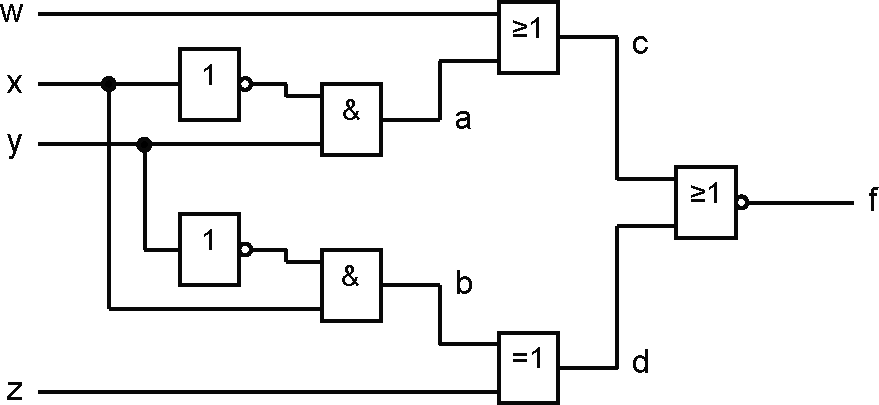
\includegraphics[scale=0.63]{pINLDIG2014_opgave5_schema.pdf}
    \caption{deel microprocessorschakeling.}
    \label{fig:opgave5}
  \end{minipage}\hfill
  \begin{minipage}[c]{.350\linewidth}
  	% Tell Latex it's a table
    \captionof{table}{Vertragingstijden}
    \label{tab:vertragingstijden}
    \begin{tabular}{ l | c c }
      \hline
          &              &               \\ [-2.9ex]
    Poort & $t_{P(min)}$ & $t_{P(max)}$  \\ \hline
    EXOR  &    4,5       &     9,7       \\
    AND   &    2,4       &     6,9       \\
    OR    &    3,1       &     7,2       \\
    NOR   &    2,5       &     6,0       \\
    NOT   &    1,5       &     4,3       \\
    \end{tabular}
    \vskip10pt
  \end{minipage}\hfill
\end{figure}

\begin{parts}
\part[5] \label{opg:opg5a} Bepaal de minimale en maximale vertragingstijden
van de gehele schakeling. Laat de berekeningen zien {} \droppoints{}.
\part[10] \label{opg:opg5b} Reken deze schakeling door en bepaal de logische
functie in mintermvorm (ook wel canonieke vorm genoemd). Hint: stel
een waarheidstabel op voor alle interne knooppunten, zodat de functie
makkelijk te vinden is uit de functiewaarden van deze interne knooppunten {}
\droppoints{}.
\end{parts}


\newpage

\question[10]
\label{opg:opg6}
Gegeven onderstaande flipflopschakeling (figuur \ref{fig:opg6}). De beginstand van de
flipflop is 0.

\begin{figure}[H]
  \centering
  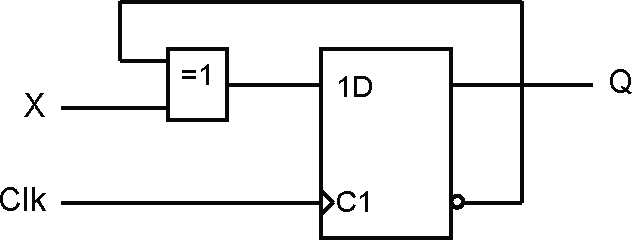
\includegraphics[scale=0.63]{pINLDIG2014_opgave6_schema.pdf}
  \caption{Flipflopschakeling.}
  \label{fig:opg6}
\end{figure}

Op ingang $Clk$ worden 12 klokpulsen aangeboden. Op ingang $X$ wordt het
volgende bitpatroon aangeboden: $011101001101$ (beginnend met de linker $0$),
elke (bit-)waarde steeds vlak
voor de opgaande flank. Geef bij elke (bit-)waarde van ingang $X$ vlak voor de
opgaande flank van ingang $Clk$ steeds de (bit-)waarde van uitgang $Q$ vlak na
de opgaande flank van ingang $Clk$. Timing wordt buiten beschouwing gelaten.



\question
\label{opg:opg7}
Gegeven een poging tot het ontwerpen van een latch. Zie figuur \ref{fig:opg7}.

\begin{figure}[H]
  \centering
  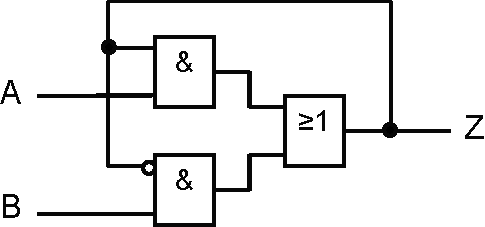
\includegraphics[scale=0.63]{pINLDIG2014_opgave7_schema.pdf}
  \caption{Latch.}
  \label{fig:opg7}
\end{figure}

\begin{parts}
\part[5] \label{opg:opg7a} Geef de logische functie van $Z$ uitgedrukt in $A$ en $B$ {} \droppoints{}.
\part[7] \label{opg:opg7b} Bepaal wat voor functie de vier combinaties van $A$ en $B$ hebben m.b.t. de latch. Stel
hiervoor een waarheidstabel op {} \droppoints{}.
\part[3] \label{opg:opg7c} Is dit een praktische, bruikbare latch? Motiveer het antwoord {} \droppoints{}.
\end{parts}


\vspace{4em}
\begin{center}
o-o-o-o- einde toets -o-o-o-o-
\end{center}




\ifprintanswers
\newpage
\textbf{Uitwerking opgave \ref{opg:opg1}}

(Opgave \ref{opg:opg1a}) Het binaire getal $0101111_{2}$ begint met een $0$ dus het getal is positief.
Daarom kan het getal in \'{e}\'{e}n keer omgezet worden naar het decimale equivalent:
\begin{equation*}
\begin{split}
0101111_{2} &= 0 \cdot 2^{6} + 1 \cdot 2^{5} + 0 \cdot 2^{4} + 1 \cdot 2^{3} 1 \cdot 2^{2} + 1 \cdot 2^{1} + 1 \cdot 2^{0} \\
            &= 2^{5} + 2^{3} + 2^{2} + 2^{1} + 2^{0} \\
            &= 32 + 8 + 4 + 2 + 1 \\
            &= 47_{10}
\end{split}
\end{equation*}
(Opgave \ref{opg:opg1b}) Het hexadecimale getal $8000_{16}$ verdient wat meer aandacht. In feite is de
hexadecimale schrijfwijze een notatie om het aantal te schrijven bits te verminderen. Een hexadecimaal
getal is dus eenvoudig als binair getal te schrijven door elk hexadecimaal cijfer weer te geven met
precies vier bits: $8000_{16} = 1000.0000.0000.0000_{2}$. Nu is goed
te zien dat het binaire getal begint met een $1$, dus het betreft een negatief getal.

Het getal is direct naar het decimale talstelsel om te schrijven door het meest significante bit
als negatief te zien:
\begin{equation*}
8000_{16} = 1000.0000.0000.0000_{2} = -1 \cdot 2^{15} = -32768_{10}
\end{equation*}

(Opgave \ref{opg:opg1c}) Het omzetten geschiedt door herhaald vermenigvuldigen
met twee en steeds het gehele deel te noteren en verder te gaan met de fractie.
Hieronder de uitwerking:

\begin{table}[H]
  %\label{table:ant_opgave3b}
  \begin{tabular}{ r c c r c c }
  0,45 & x 2 & = & 0,9 & $\rightarrow$ & 0 \\
   0,9 & x 2 & = & 1,8 & $\rightarrow$ & 1 \\
   0,8 & x 2 & = & 1,6 & $\rightarrow$ & 1 \\
   0,6 & x 2 & = & 1,2 & $\rightarrow$ & 1 \\
   0,2 & x 2 & = & 0,4 & $\rightarrow$ & 0 \\
   0,4 & x 2 & = & 0,8 & $\rightarrow$ & 0 \\
   \underline{0,8} &     &   &     &               &
  \end{tabular}
\end{table}

Nu is goed te zien dat de laatste vier bits zich blijven herhalen. Dus
$0,45_{10} = 0,01\underline{1100}...._{2}$ waarbij de onderstreping het
zich herhalende deel aangeeft. Dat houdt ook in dat $0,45_{10}$ dus niet
exact kan worden weergegeven in het binaire systeem.

Voor afronding moet worden gekeken naar het eerste binaire cijfer na het
aantal weer te geven binaire cijfers. Als dat een 1 is, dan moet naar
boven worden afgerond, is het een 0 dan moet naar beneden worden afgerond.
In dit geval is het een 1 (zie onderstreping), dus er moet naar boven worden
afgerond.
\begin{equation*}
\begin{split}
0,45_{10} &= 0,0111001100|\underline{1}100..._{2} \\
          &= 0,0111001101_{2} \qquad \qquad \text{(na afronding)}
\end{split}
\end{equation*}
(Opgave \ref{opg:opg1d}) De kleinste waarde is $-89,2\ ^{\circ}$C en wordt
dus weergegeven als $-892$. De grootste waarde is $+57,7\ ^{\circ}$C en wordt
weergegeven als $577$. De waarde $0,0\ ^{\circ}$C wordt weergegeven als $0$,
er is dus geen offset. Voor de kleinste waarde zijn minimaal
$\lceil ^{2}\log\,(892+1) \rceil = \lceil 9,80\ldots \rceil = 10$ bits nodig.
Voor de grootste waarde zijn $\lceil ^{2}\log\,(577+1) \rceil = \lceil 
9,17\ldots \rceil = 10$ bits nodig. Omdat er zowel positieve als negatieve
getallen gebruikt worden is er nog een tekenbit nodig. Het benodigde aantal
bits is dus 11.


\newpage
\textbf{Uitwerking opgave \ref{opg:opg2}}

(Opgave \ref{opg:opg2a}) De functie wordt ingevuld in een Karnaughdiagram en daarna
uitgewerkt, zie figuur~\ref{fig:ant_opgave2a_kmaps}.

\begin{figure}[H]
  \begin{minipage}[c]{0.50\linewidth}
    \centering
	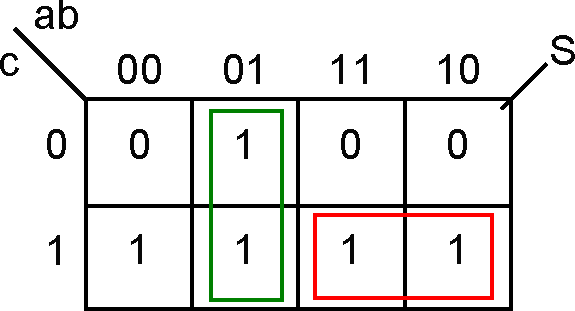
\includegraphics[scale=0.50]{pINLDIG2014_opgave2a_kmaps.pdf}
    \caption{Karnaughdiagram voor functie S.}
    \label{fig:ant_opgave2a_kmaps}
  \end{minipage}
  \begin{minipage}[c]{.40\linewidth}
  De groene omranding levert de term $\oline{a} \cdot b$ op en de rode
  omranding levert de term $a \cdot c$ op. De functie voor S is dus
  \begin{equation*}
  S = \oline{a} \cdot b + a \cdot c
  \end{equation*}
  \end{minipage}\hfill
\end{figure}

(Opgave \ref{opg:opg2b}) De functie S moet worden omgezet zodat deze volledig
wordt uitgedrukt in NAND-termen. Dat kan door het toepassen van de wetten van
De Morgan:
\begin{equation*}
S = \oline{a} \cdot b + a \cdot c = \oline{\oline{\oline{a} \cdot b} \, \cdot \, \oline{a \cdot c}}
\end{equation*}

(Opgave \ref{opg:opg2c}) Het schema dat uit opgave \ref{opg:opg2b}) volgt kan
dan als volgt getekend worden, zie figuur~\ref{fig:ant_opgave2c_schema}:

\begin{figure}[H]
  \centering
  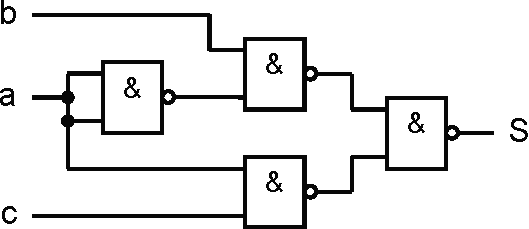
\includegraphics[scale=0.63]{pINLDIG2014_opgave2c_schema.pdf}
  \caption{Schema voor functie S met alleen NANDs.}
  \label{fig:ant_opgave2c_schema}
\end{figure}


\vspace{1em}

\textbf{Uitwerking opgave \ref{opg:opg3}}

(Opgave \ref{opg:opg3a}) Eerst moeten beide getallen postief gemaakt worden.
Dat is niet zo heel moeilijk. Het omzetten naar binair geschiedt door herhaald
delen door twee en steeds de rest na deling te te noteren en verder te gaan
met het gehele deel. Hieronder de uitwerking:

\begin{table}[H]
  %\label{table:ant_opgave3b}
  \begin{tabular}{ r c c r c c }
  105 & $\div$ 2 & = & 52 r 1 & $\rightarrow$ & 1 \\
   52 & $\div$ 2 & = & 26 r 0 & $\rightarrow$ & 0 \\
   26 & $\div$ 2 & = & 13 r 0 & $\rightarrow$ & 0 \\
   13 & $\div$ 2 & = &  6 r 1 & $\rightarrow$ & 1 \\
    6 & $\div$ 2 & = &  3 r 0 & $\rightarrow$ & 0 \\
    3 & $\div$ 2 & = &  1 r 1 & $\rightarrow$ & 1 \\
    1 & $\div$ 2 & = &  0 r 1 & $\rightarrow$ & 1 \\
   \underline{0} &   &  &     &               &
  \end{tabular}
\end{table}

Het getal $105_{10}$ is dus gelijk aan $01101001_{2}$. Let op de extra 0
vooraan het getal. Dit is om het getal positief te houden. Het getal $15_{10}$ is op
vergelijkbare wijze om te zetten en dat levert $01111_{2}$ op.
Beide getallen staan nu als positief getal genoteerd, en moeten negatief
gemaakt worden. Dat kan door middel van \textit{flip bits, add one}.

\begin{table}[H]
  \begin{tabular}{ r l c c r l  }
   01101001 & $(+105)$  & & & 01111 & $(+15)$   \\
            &           & & &       &           \\
   10010110 & flip bits & & & 10000 & flip bits \\
          1 & +         & & &     1 & +         \\  \cline{1-1} \cline{5-5}
   10010111 & $(-105)$  & & & 10001 & $(-15)$
  \end{tabular}
\end{table}

Nu moeten beide getallen nog naar 8-bits formaat worden uitgebreid. Het getal
$10010111_{2}$ is al in 8-bits formaat, dus uitbreiding is niet nodig. Het
getal $10001_{2}$ moet aangevuld worden met 1-en, dus $11110001_{2}$. Dus:
\begin{eqnarray}
\nonumber -105_{10} & = & 10010111_{2} \\
\nonumber -15_{10}  & = & 11110001_{2}
\end{eqnarray}
Overigens kan ook eerst tekenuitbreiding uitgevoerd worden en daarna
negatief maken, het resultaat blijft hetzelfde.

(Opgave \ref{opg:opg3b}) Het optellen van de twee getallen is niet zo lastig,
ook al zijn het negatieve getallen. De normale optelprocedure kan gebruikt
worden (daarom is het 2's complement ook bedacht).

\begin{table}[H]
  \begin{tabular}{ r c l }
   1)11101110 &   & carry's     \\
     10010111 &   & -105        \\
     11110001 & + & -15         \\  \cline{1-1}
   1)10001000 &   & -120    
  \end{tabular}
\end{table}

De uitgaande carry mag verwaarloosd worden, die is geen onderdeel van het antwoord.
De carry is het resultaat van de wijze waarop het 2's complementsysteem werkt.


\vspace{1em}

\textbf{Uitwerking opgave \ref{opg:opg4}}

(Opgave \ref{opg:opg4a}) Eerst moet de waarheidstabel worden opgezet. De
bitcombinaties $A = a_{1}a_{0}$ kunnen gezien worden als een
getal dat ligt tussen 0 en 3: $a_{1}a_{0} = 00 = 0$, $a_{1}a_{0} = 01 = 1$,
$a_{1}a_{0} = 10 = 2$ en $a_{1}a_{0} = 11 = 3$. Dat kan zo ook met
$B = b_{1}b_{0}$. De functie moet de maximale waarde geven van de bitcombinaties
tussen $a_{1}a_{0}$ en $b_{1}b_{0}$ en weergeven met de bits $M = m_{1}m_{0}$.
Neem als voorbeeld $A = a_{1}a_{0} = 01$ en $B = b_{1}b_{0} = 10$, dan is de uitkomst
$M = m_{1}m_{0} = 10$, want $B$ is groter dan $A$. Van alle mogelijkheden
wordt een waarheidstabel opgezet, die is te vinden in tabel \ref{tab:ant_opgave4a}.

(Opgave \ref{opg:opg4b}) Nadat de waarheidstabel is opgezet, moeten de functies
in Karnaughdiagrammen ingevoerd en uitgewerkt worden. Dit is weergegeven in
figuur \ref{fig:ant_opgave4b_kmaps}. De gevonden functies voor $m_{1}$ en $m_{0}$
zijn
\begin{equation*}
\begin{split}
m_{1} & = a_{1} + b_{1} \\
m_{0} & = a_{1} \cdot a_{0} + b_{1} \cdot b_{0} + \oline{a_{1}} \cdot b_{0} + a_{0} \cdot \oline{b_{1}}
\end{split}
\end{equation*}

(Opgave \ref{opg:opg4c}) De schema's van de twee functies zijn weergegeven
in figuur \ref{fig:ant_opgave4c_schema}.

\begin{figure}[H]
  \begin{minipage}[c]{.30\linewidth}
    \captionof{table}{Waarheidstabel voor de functies $m_{1}$ en $m_{0}$.}
    \label{tab:ant_opgave4a}
    \begin{tabular}{ c c c c | c  c }
      \hline
              &         &         &         &         &         \\ [-2.9ex]
      $a_{1}$ & $a_{1}$ & $b_{1}$ & $b_{0}$ & $m_{1}$ & $m_{0}$ \\ \hline
         0    &    0    &    0    &    0    &    0    &    0   \\
         0    &    0    &    0    &    1    &    0    &    1   \\
         0    &    0    &    1    &    0    &    1    &    0   \\
         0    &    0    &    1    &    1    &    1    &    1   \\ \hdashline
         0    &    1    &    0    &    0    &    0    &    1   \\
         0    &    1    &    0    &    1    &    0    &    1   \\
         0    &    1    &    1    &    0    &    1    &    0   \\ 
         0    &    1    &    1    &    1    &    1    &    1   \\ \hdashline
         1    &    0    &    0    &    0    &    1    &    0   \\
         1    &    0    &    0    &    1    &    1    &    0   \\
         1    &    0    &    1    &    0    &    1    &    0   \\
         1    &    0    &    1    &    1    &    1    &    1   \\ \hdashline
         1    &    1    &    0    &    0    &    1    &    1   \\
         1    &    1    &    0    &    1    &    1    &    1   \\
         1    &    1    &    1    &    0    &    1    &    1   \\ 
         1    &    1    &    1    &    1    &    1    &    1   \\ \hline
    \end{tabular}
    \vskip10pt
  \end{minipage}\hfill
  \begin{minipage}[c]{0.65\linewidth}
    \centering
	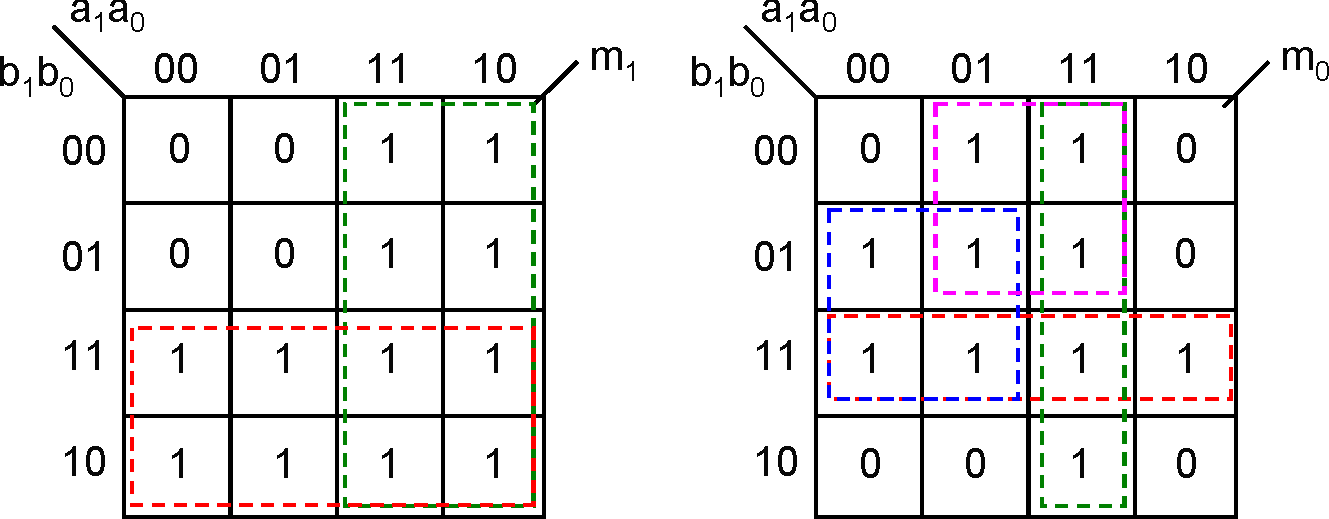
\includegraphics[scale=0.50]{pINLDIG2014_opgave4b_kmaps.pdf}
    \caption{Karnaughdiagrammen voor de functies $m_{1}$ en $m_{0}$.}
    \label{fig:ant_opgave4b_kmaps}
  \end{minipage}
\end{figure}

\begin{figure}[H]
  \centering
  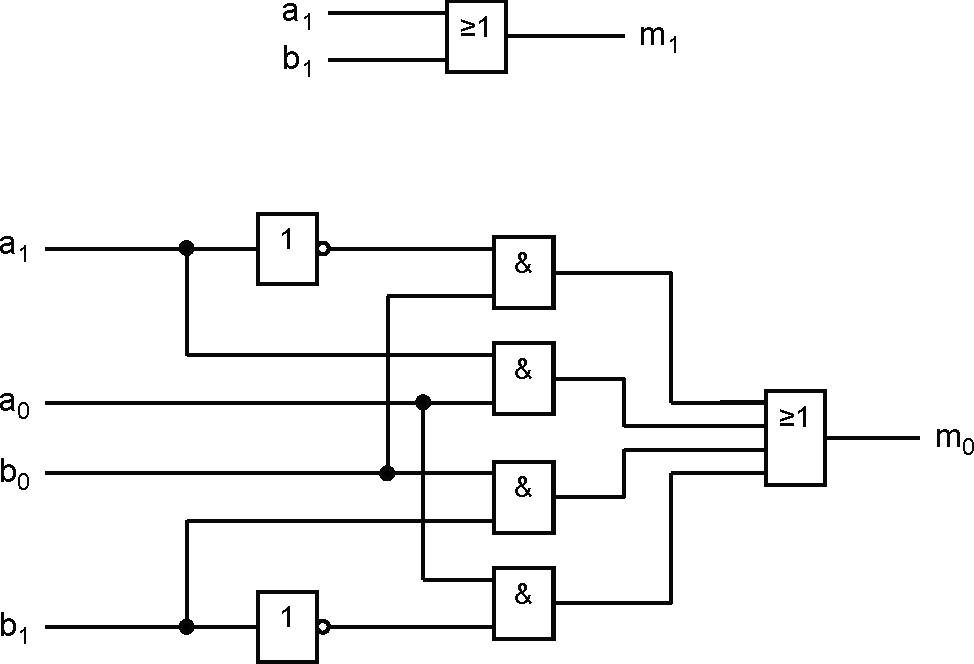
\includegraphics[scale=0.63]{pINLDIG2014_opgave4c_schema.pdf}
  \caption{Schema's voor functies $m_{1}$ en $m_{0}$.}
  \label{fig:ant_opgave4c_schema}
\end{figure}


\newpage
\textbf{Uitwerking opgave \ref{opg:opg5}}

(Opgave \ref{opg:opg5a}) Het berekenen van de minimale propagatietijd is niet zo lastig.
Snel is te zien dat het korste pad (in tijd) via de ingangen $w$ of $z$ verloopt. Via $w$
wordt een OR-poort gepasseerd naar intern knooppunt $c$ en dan via een NOR-poort naar
uitgang $f$. Vanuit $z$ wordt een EXOR-poort gepasseerd naar intern knooppunt $d$ en
dan dan via een NOR-poort naar uitgang $f$. De OR-poort heeft minder vertraging dan de
EXOR-poort. Het korste pad is dus $w \rightarrow c \rightarrow f$. De minimale
propagatietijd is dan
\begin{equation*}
t_{P(min)}(f) = t_{P(min)}(\text{OR}) + t_{P(min)}(\text{NOR}) = 3,1 + 2,5 = 5,6 \, \textrm{ns}
\end{equation*}

Voor het berekenen van de maximale propagatietijd is wat meer werk nodig. Er moet nu
gezocht worden naar het langste pad (in tijd). De ingangen $w$ en $z$ geven zeker niet
de maximale tijd, hiervoor moet gestart worden met ingangen $x$ en $y$. Signalen via
$x$ komen via een inverter en een AND-poort aan bij interne knooppunt $a$. Dezelfde
opzet is te zien voor ingang $y$ naar intern signaal $b$. Tot hier is de propagatietijd even
groot. Daarna kan gekozen worden via intern knooppunt $c$ en $d$. Via $d$ wordt een
EXOR-poort gepasseerd en die heeft meer vertraging dan de OR-poort. Het pad voor de maximale
propagatietijd is dus $y \rightarrow b \rightarrow d \rightarrow f$:
\begin{equation*}
\begin{split}
t_{P(max)}(f) &= t_{P(max)}(\text{NOT}) + t_{P(max)}(\text{AND}) + t_{P(max)}(\text{EXOR}) + t_{P(min)}(\text{NOR}) \\
              &= 4,3 + 6,9 + 9,7 + 6,0 = 26,9 \, \textrm{ns}
\end{split}
\end{equation*}

(Opgave \ref{opg:opg5b}) Het doorrekenen van de schakeling kan het best via het opstellen
van een waarheidstabel uitgevoerd worden. Daarbij spelen de interne knooppunten een
belangrijke rol. Dit zijn eenvoudige functies waarvan de logische werking bekend is.
De interne knooppunten vormen op hun beurt weer ingangen voor een aantal functies.
Er is een waarheidstabel op te stellen voor de ingangen, de interne knooppunten en de
uitgang. Deze is te vinden in tabel \ref{tab:ant_opgave5b}.

\begin{table}[H]
  \caption{Waarheidstabel voor de schakeling uit figuur \ref{fig:opgave5}}
  \label{tab:ant_opgave5b}
    \begin{tabular}{ c c c c | c c c c | c }
      \hline
            &         &         &         &         &         &         &         &       \\ [-2.9ex]
      $w$   &   $x$   &   $y$   &   $z$   &   $a$   &   $b$   &   $c$   &   $d$   & $f$   \\ \hline
       0    &    0    &    0    &    0    &    0    &    0    &    0    &    0    &  1    \\
       0    &    0    &    0    &    1    &    0    &    0    &    0    &    1    &  0    \\
       0    &    0    &    1    &    0    &    1    &    0    &    1    &    0    &  0    \\
       0    &    0    &    1    &    1    &    1    &    0    &    1    &    1    &  0    \\ \hdashline
       0    &    1    &    0    &    0    &    0    &    1    &    0    &    1    &  0    \\
       0    &    1    &    0    &    1    &    0    &    1    &    0    &    0    &  1    \\
       0    &    1    &    1    &    0    &    0    &    0    &    0    &    0    &  1    \\ 
       0    &    1    &    1    &    1    &    0    &    0    &    0    &    1    &  0    \\ \hdashline
       1    &    0    &    0    &    0    &    0    &    0    &    1    &    0    &  0    \\
       1    &    0    &    0    &    1    &    0    &    0    &    1    &    1    &  0    \\
       1    &    0    &    1    &    0    &    0    &    0    &    1    &    0    &  0    \\
       1    &    0    &    1    &    1    &    0    &    0    &    1    &    1    &  0    \\ \hdashline
       1    &    1    &    0    &    0    &    1    &    0    &    1    &    0    &  0    \\
       1    &    1    &    0    &    1    &    1    &    0    &    1    &    1    &  0    \\
       1    &    1    &    1    &    0    &    0    &    0    &    1    &    0    &  0    \\ 
       1    &    1    &    1    &    1    &    0    &    0    &    1    &    1    &  0    \\ \hline
    \end{tabular}
\end{table}

De functie is
\begin{equation*}
f = m_{0} + m_{5} + m_{7} = \sum m(0,5,7)
\end{equation*}


\vspace{1em}

\textbf{Uitwerking opgave \ref{opg:opg6}}

De D-ingang wordt aangestuurd door een EXOR van $X$ en de inverse van $Q$. Er
kan een waarheidstabel worden opgesteld voor de waarde die aan D wordt
aangeboden. Zie tabel \ref{tab:opg6_xor}.

\begin{table}[H]
  \begin{minipage}[c]{0.40\linewidth}
    \caption{Waarheidstabel voor functie $D$.}
    \label{tab:opg6_xor}
    %\centering
	\begin{tabular}{c c | c}
	\hline
              &         &               \\ [-2.9ex]
      $X^{n}$ & $Q^{n}$ & $D^{n}$       \\ \hline
        0     &   0     &   1           \\
        0     &   1     &   0           \\
        1     &   0     &   0           \\
        1     &   1     &   1           \\ \hline
	\end{tabular}	    
  \end{minipage}
  \begin{minipage}[c]{.60\linewidth}
  \begin{equation}
  \nonumber D^{n} = X^{n} \oplus \oline{Q^{n}} = \oline{X^{n} \oplus Q^{n}}
  \end{equation}
  \end{minipage}\hfill
\end{table}

De flipflop heeft eerst de stand 0. De eerste waarde die aangeboden wordt is
ook 0. Uit de tabel volgt dat $D$ dus logisch 1 wordt. Zo moeten alle waarden
van $X$ worden afgegaan, steeds uitrekenen wat de waarde van $Q$ wordt. Er
wordt een tabel opgesteld met $X^{n}$, $Q^{n}$, $D^{n}$ en $Q^{n+1}$. Merk op
dat $Q^{n+1} = D^{n}$ want dat is de werking van een D-flipflop. Zie tabel
\ref{tab:ant_opg6}.

\begin{table}[H]
  \caption{Doorlopen standen van de flipflop.}
  \label{tab:ant_opg6}
  \begin{tabular}{ c | c c | c c }
    \hline
         &         &         &         &            \\ [-2.9ex]
     nr. & $X^{n}$ & $Q^{n}$ & $D^{n}$ & $Q^{n+1}$  \\ \hline
      1  &    0    &    0    &    1    &    1       \\
      2  &    1    &    1    &    1    &    1       \\
      3  &    1    &    1    &    1    &    1       \\
      4  &    1    &    1    &    1    &    1       \\
      5  &    0    &    1    &    0    &    0       \\
      6  &    1    &    0    &    0    &    0       \\
      7  &    0    &    0    &    1    &    1       \\ 
      8  &    0    &    1    &    0    &    0       \\
      9  &    1    &    0    &    0    &    0       \\
     10  &    1    &    0    &    0    &    0       \\
     11  &    0    &    0    &    1    &    1       \\
     12  &    1    &    1    &    1    &    1       \\
     13  &    1    &    -    &    -    &    -       \\ \hline
  \end{tabular}
\end{table}

\vspace{1em}

\textbf{Uitwerking opgave \ref{opg:opg7}}

(Opgave \ref{opg:opg7a}) Eerst een korte analyse van de schakeling. De OR- en
AND-poorten rechts/boven vormen een rondgekoppelde SR-latch. De AND-poort
linksonder is wat vreemd, er zit een inverter in de terugkoppeling. De
logische functie van $Z$ uitgedrukt in $A$ en $B$ is
\begin{equation*}
\begin{split}
Z_{nieuw} &= A \cdot Z_{oud} + B \cdot \oline{Z_{oud}}
\end{split}
\end{equation*}
waarbij $Z_{nieuw}$ de nieuwe gegenereerde waarde is en $Z_{oud}$ de oude
(huidige) waarde.

(Opgave \ref{opg:opg7b}) Direct is te zien dat als $AB = 00$ dat
$Z_{nieuw} = 0$ (resetten). Als $AB = 10$ dan is $Z_{nieuw} = Z_{oud}$
(onthouden).
Bij $AB = 11$ levert de functie $Z_{nieuw} = 1$ op (set). Als $AB = 01$
dan is $Z_{nieuw}$ de inverse van $Z_{oud}$, dat betekent
oscillatie: de uitgang verandert na een aantal poortvertragingen steeds
van stand. De functie van de latch kan prima in een waarheids- en
functietabel worden gezet. Zie de tabellen \ref{tab:opg7_truth_table}
en \ref{tab:opg7_function_latch}.

\begin{table}[H]
  \begin{minipage}[c]{0.50\linewidth}
  	\caption{Waarheidstabel voor functie $Z_{nieuw}$.}
	\label{tab:opg7_truth_table}
	\begin{tabular}{ c c c | c}
		\hline 
		$A$ & $B$ & $Z_{oud}$ & $Z_{nieuw}$ \\ \hline 
		 0  &  0  &   0       &   0       \\ 
		 0  &  0  &   1       &   0       \\ \hdashline
		 0  &  1  &   0       &   1       \\ 
		 0  &  1  &   1       &   0       \\ \hdashline
		 1  &  0  &   0       &   0       \\ 
		 1  &  0  &   1       &   1       \\ \hdashline
		 1  &  1  &   0       &   1       \\ 
		 1  &  1  &   1       &   1       \\ \hline 
	\end{tabular} 
  \end{minipage}
  \begin{minipage}[c]{.50\linewidth}
    \caption{Functietabel voor functie $Z_{nieuw}$.}
    \label{tab:opg7_function_latch}
	\begin{tabular}{c c | c}
	\hline
              &         &               \\ [-2.9ex]
       $A$    &  $B$    & functie       \\ \hline
        0     &   0     & reset         \\
        0     &   1     & inverse       \\
        1     &   0     & onthouden     \\
        1     &   1     & set           \\ \hline
	\end{tabular}	    
  \end{minipage}\hfill
\end{table}


(Opgave \ref{opg:opg7c}) 
De latch is te gebruiken omdat de drie benodige functies onhouden, setten en
resetten kunnen worden uitgevoerd \'{e}n de onthoudstand door slechts
\'{e}\'{e}n bitwisseling te bereiken is vanuit de set- en resetstand.

Vervelend is dat de latch oscilleert als $AB = 01$, dus deze combinatie
moet niet gebruikt worden. Verder is deze latch opgebouwd uit drie poorten
(inverter niet meegerekend) terwijl een goed werkende latch ook met twee
poorten gemaakt kan worden. In de praktijk wordt deze latch niet gebruikt.

\vspace{4em}
\begin{center}
o-o-o-o- einde uitwerkingen -o-o-o-o-
\end{center}

\fi  %% end printanswers

\end{questions}

\end{document}
